
\section{Methodology}
We simulated the nuclear reactor operating history in the \gls{EU} beginning in 
1970 including \gls{MOX} production and use in France. 
The simulation captured all discrete regions, reactor facilities, and materials 
involved in \gls{EU} historical reactor operation
using \Cyclus fuel cycle simulation framework and \Cycamore agents.
In this simulation, the \gls{UNF} from \gls{EU} nations is stored for later use 
in French \glspl{SFR} and France begins production of fuel for \glspl{SFR}
in 2020 by recycling the stored \gls{UNF}.
The \glspl{SFR} are modeled after the \gls{ASTRID} breeder reactor \cite{varaine_pre-conceptual_2012}.

All scripts and data used for the simulations in this article are available in 
\cite{bae_arfc/transition-scenarios:_2017}.


\subsection{\Cyclus}

\Cyclus is an agent-based fuel cycle simulation framework 
\cite{huff_fundamental_2016}, which means 
that each reactor, reprocessing plant, and fuel fabrication plant is modeled as an agent.

A \Cyclus simulation contains prototypes, which are fuel cycle facilities with
pre-defined parameters, that are deployed in the simulation as \texttt{facility} agents.
Encapsulating the \texttt{facility} agents are the \texttt{Institution} and \texttt{Region}.
A \texttt{Region} agent holds a set of \texttt{Institution}s. 
An \texttt{Institution} agent can deploy or decommission \texttt{facility} agents.
The \texttt{Institution} agent is part of a \texttt{Region} agent,
which can contain multiple \texttt{Institution} agents. Several versions of \texttt{Institution}
and \texttt{Region} exist, varying in complexity and functions \cite{huff_extensions_2014}.
 \texttt{DeployInst} is used as the institution archetype for this work, where the institution
deploys agents at user-defined timesteps. 

At each timestep (one month),
agents make requests for materials or bid to supply them and exchange
with one another. A market-like mechanism called the dynamic resource exchange
\cite{gidden_agent-based_2015} governs the exchanges.
Each material resource has a quantity, composition, name, and a unique identifier
for output analysis. 

In this work, each nation is represented as a distinct \texttt{Region} agent,
that may contain \texttt{Institution} agents, each deploying  \texttt{Facility} 
agents. The \texttt{Institution} agents then deploy agents according to 
a user-defined deployment scheme.


\subsection{Nuclear Deployment in the \gls{EU}}


The \gls{IAEA} \gls{PRIS} database \cite{iaea_pris_2017} contains worldwide reactor
operation history.
We import this database directly as a csv file, to populate the simulation
with deployment information, listing the country, reactor unit, type, net capacity (\gls{MWe}), status,
operator, construction date, first criticality date, first grid date, commercial date, shutdown
date (if applicable), and unit capacity factor for 2013. Then only the \gls{EU} countries are extracted
from the csv file. We developed a python script to generate a \Cyclus input file from the csv file,
which lists the individual reactor units as agents. 


\begin{figure}
        \centering
        \scalebox{0.7}{
\begin{tikzpicture}[node distance=1.5cm]
\node (database) [object] {Database (\texttt{.csv})};
\node (script) [process, below of=database] {Input Generation Script (\texttt{write\_deployinst\_input.py})};
\node (input) [object, below of=script] {\Cyclus Input File (\texttt{.xml})};
\node (cyclus) [process, below of=input]{\Cyclus};
\node (output) [object, below of=cyclus]{\texttt{Output File (\texttt{.Sqlite})}};
\node (script2) [process, below of=output]{Analysis Script (\texttt{analysis.py})};

\draw [arrow] (database) -- (script); 
\draw [arrow] (script) -- (input); 
\draw [arrow] (input) -- (cyclus);
\draw [arrow] (cyclus) -- (output);
\draw [arrow] (output) -- (script2);
\end{tikzpicture}
}
\caption{Computational workflow in this work. The green circles represent files, and the blue
         boxes represent codes that process the files.}
\label{diag:comp}
\end{figure}


Projections of future reactor deployment in this simulation are based on
assessment of analyses from references such as \gls{PRIS} for reactors planned
for construction \cite{iaea_pris_2017}, the World Nuclear Association
\cite{world_nuclear_association_nuclear_2017}, and literature concerning the future of
nuclear power in a global \cite{joskow_future_2012} and European context
\cite{hatch_politics_2015}.  Existing projections extend to 2050 at the latest.  

\Cref{tab:eu_deployment} lists the reactors that are currently  planned or
under construction. In the simulation, all  planned constructions are completed 
without delay or failure and are assumed to reach a lifetime of 60 years.  

\begin{table}[h]
    \centering

    \label{tab:eu_deployment}
    \scalebox{0.9}{
    \begin{tabular}{ccccr}
        \hline
        \textbf{Exp. Operational }&\textbf{Country} &\textbf{Reactor} & \textbf{Type} & \textbf{Gross \gls{MWe}}\\
        \hline
        2018 & Slovakia  & Mochovce 3 & PWR & 440\\
        2018 & Slovakia & Mochovce 4 & PWR & 440 \\
        2018 & France & Flamanville 3 & PWR & 1600 \\
        2018 & Finland & Olkilouto 3 & PWR & 1720 \\
        2019 & Romania & Cernavoda 3 & PHWR & 720 \\
        2020 & Romania & Cernavoda 4 & PHWR & 720 \\
        2024 & Finland & Hanhikivi & VVER1200 & 1200 \\
        2024 & Hungary & Paks 5 & VVER1200 & 1200 \\
        2025 & Hungary & Paks 6 & VVER1200 & 1200 \\
        2025 & Bulgaria & Kozloduy 7 & AP1000 & 950 \\
        2026 & UK & Hinkley Point C1 & EPR & 1670 \\
        2027 & UK & Hinkley Point C2 & EPR & 1670 \\
        2029 & Poland & Choczewo & N/A & 3000 \\
        2035 & Poland & N/A & N/A & 3000 \\
        2035 & Czech Rep & Dukovany 5 & N/A & 1200 \\
        2035 & Czech Rep & Temelin 3 & AP1000 & 1200 \\
        2040 & Czech Rep & Temelin 4 & AP1000 & 1200 \\
        \hline
    \footnote{The fate of many planned reactors are uncertain. The proposed reactor types
              are also unclear. The ones marked `N/A' for type are assumed to the \glspl{PWR}
              in the simulation.}
    \end{tabular}
    }
    \label{tab:eu_deployment}
    \caption {Power Reactors under construction and planned.
        Replicated from \cite{world_nuclear_association_nuclear_2017}.}
\end{table}
\FloatBarrier

For each \gls{EU} nation, we categorize the growth trajectory is categorized from
``Aggressive Growth'' to ``Aggressive Shutdown''. Aggressive growth is
characterized by a rigorous expansion of nuclear power while
Aggressive Shutdown is characterized as a transition to rapidly
de-nuclearize the nation's electric grid. A nation's growth trajectory is
categorized into five degrees depending on G, the growth trajectory metric.

 \[
 G = \left\{\begin{array}{ll}
 \text{Aggressive Growth}, & \text{for } G \geq 2\\
 \text{Modest Growth}, & \text{for } 1.2 \leq G < 2\\
 \text{Maintanence}, & \text{for } 0.8 \leq G < 1.2 \\
 \text{Modest Reduction}, & \text{for } 0.5 \leq G< 0.8\\
 \text{Aggressive Reduction}, & \text{for } G \leq 0.5
 \end{array}\right\} = \frac{C_{2040}}{C_{2017}}\\\\
 \]
 \[
  G = \text{Growth Trajectory  } [-] 
 \]
 \[
 C_{i} = \text{Nuclear Capacity in Year i  } [\gls{MWe}]
 \]

The growth trajectory and specific plan of each nation in the \gls{EU} 
is listed in Table \ref{tab:eu_growth}. Meanwhile, \cref{fig:eu_pow} displays the
timeseries of installed capacity in \gls{EU} nations.


\begin{table}[h]
    \centering
        \begin{tabular}{lll}
            \hline 
                    \textbf{Nation} & \textbf{Growth Trajectory} & \textbf{Specific Plan }\\
                    \hline
                    UK & Aggressive Growth & {\small  13 units (17,900 \gls{MWe}) by 2030.}\\
                    Poland & Aggressive Growth &  {\small Additional 6,000 \gls{MWe} by 2035.}\\
                    Hungary & Aggressive Growth &  {\small Additional 2,400 \gls{MWe} by 2025.} \\ 
                    Finland & Modest Growth &  {\small Additional 2,920 \gls{MWe} by 2024.}\\
                    Slovakia & Modest Growth & {\small Additional 942 \gls{MWe} by 2025.}\\
                    Bulgaria & Modest Growth &  {\small Additional 1,000 \gls{MWe} by 2035.} \\
                    Romania & Modest Growth &  {\small Additional 1,440 \gls{MWe} by 2020.} \\
                    Czech Rep. & Modest Growth & {\small  Additional 2,400 \gls{MWe} by 2035.}\\
                    France & Modest Reduction & {\small No expansion or early shutdown.}\\
                    Slovenia & Modest Reduction & {\small No expansion or early shutdown.}\\
                    Netherlands & Modest Reduction & {\small No expansion or early shutdown.}\\
                    Lithuania & Modest Reduction & {\small No expansion or early shutdown.}\\
                    Spain & Modest Reduction &  {\small No expansion or early shutdown.} \\
                    Italy & Modest Reduction & {\small No expansion or early shutdown. }\\
                    Belgium & Aggressive Reduction & All shut down 2025.\\
                    Sweden & Aggressive Reduction & All shut down 2050.\\
                    Germany & Aggressive Reduction & All shut down by 2022.\\
                    \hline
                    
        \end{tabular}

    \caption {Future Nuclear Programs of \gls{EU} Nations \cite{world_nuclear_association_nuclear_2017}}
  \label{tab:eu_growth}
\end{table}
\FloatBarrier

\begin{figure}[htbp!]
    \begin{center}
        \includegraphics[scale=0.6]{./images/eu_future/power_plot.png}
    \end{center}
    \caption{The timeseries of installed nuclear capacity in the EU is separated by \texttt{Region}s in \Cyclus.
             The sudden drops in capacity are caused by nuclear phaseout plans by nations such as Germany and Belgium.
             The predictions into the future are made to the farthest planned future.
             }
    \label{fig:eu_pow}
\end{figure}


\subsection{French \gls{SFR} Deployment Schedule}

\Cref{fig:sfr_num} and \ref{fig:dep} display
the French transition to \glspl{SFR} modeled in this simulation.
Starting in 2040, France deploys 600-\gls{MWe} \glspl{SFR} to make up for 
decommissioned French \gls{LWR} capacity. This results in an installed 
\gls{SFR} 
capacity of 66,000 \gls{MWe} by 2078 when the final \gls{LWR} is 
decommissioned. 

\begin{figure}[htbp!]
        \begin{center}
                \includegraphics[scale=0.6]{./images/french-transition/power_plot.png}
        \end{center}
        \caption{This plot shows the potential French transition from \glspl{LWR} to \glspl{SFR}.
                 The aggressive growth of nuclear in the 1980s leads to a substantial shutdown
                 of nuclear in the 2040s, which, in the simulation, are replaced by new 
                 \glspl{SFR}. The net capacity is kept at a constant of 66 GWe.}
        \label{fig:sfr_num}
\end{figure}
\begin{figure}[htbp!]
    \begin{center}
        \includegraphics[scale=0.6]{./images/french-transition/sfr_deploy.png}
    \end{center}
    \caption{The deployment of \glspl{SFR} in France is characterized by a period of
             aggressive building. An average of four reactors are built per year to
             make up for the decommissioned power plants built in the 1980s and 1990s.
             The second period of aggressive building occurs when the first generation
             of \glspl{SFR} decommission after 80 years.}
    \label{fig:dep}
\end{figure}

\begin{figure}[htbp!]
    \begin{center}
        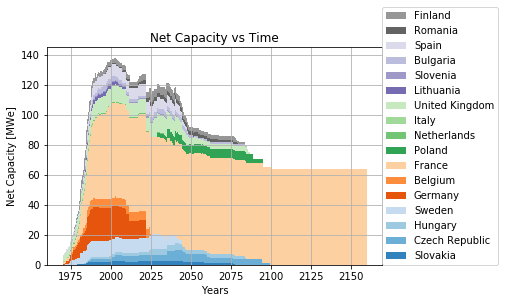
\includegraphics[scale=0.6]{./images/eu_future/onesim.png}
    \end{center}
    \caption{The total deployment scheme of the simulation. The historical
             operation \gls{EU} reactors is followed by the French
             transition to \glspl{SFR}.}
    \label{fig:tot_dep}
\end{figure}


\Cref{fig:tot_dep} displays the total deployment
scheme of the simulation.
The steep transition from 2040 to 2060 reflects the scheduled
decommissioning of reactors built in the 1975-2000
era of aggressive nuclear growth in France.

These figures reflect that, for the given assumptions, bursts of construction
are necessary to maintain capacity.  In reality, a construction rate of five 
reactors every year is highly unrealistic. However, this analysis is to analyze 
material flow, and demonstrates that, if such an aggressive deployment scheme 
took place, the \glspl{SFR} would have enough fuel.  More realistically, the 
deployment of new \glspl{SFR} can be spread out by staggering scheduled 
decommissioning of \glspl{LWR} through lifetime extensions.  An analysis of the 
effect of \gls{LWR} lifetime extension is discussed in Section \ref{sec:life}.

\subsection{Material Flow}

The fuel cycle is represented by a series of facility agents whose material 
flow is illustrated in figure \ref{diag:fc}, along with
the \Cyclus archetypes that were used to model each facility.

% Define block styles
\tikzstyle{decision} = [diamond, draw, fill=blue!20, 
text width=4.5em, text badly centered, node distance=3cm, inner sep=0pt]
\tikzstyle{block} = [rectangle, draw, fill=blue!20, 
text width=5em, text centered, rounded corners, minimum height=4em]
\tikzstyle{line} = [draw, -latex']
\tikzstyle{cloud} = [draw, ellipse,fill=red!20, node distance=3cm,
minimum height=2em]


\begin{figure}
        \centering
        \scalebox{0.6}{
                \begin{tikzpicture}[align=center, node distance = 3cm and 3cm, auto]
                % Place nodes
                \node [block] (sr) {Mine (\texttt{SOURCE})};
                \node [cloud, below of=sr] (nu) {Nat U};
                \node [block, below of=nu] (enr) {Enrichment ({\footnotesize \texttt{ENRICHMENT}})};
                \node [cloud, below of=enr] (uox) {\gls{UOX}};
                \node [block, below of=uox] (lwr) {\gls{LWR} (\texttt{REACTOR})};
                \node [cloud, right of=lwr] (snf) {\gls{UNF}};
                \node [cloud, right of=uox] (cunf) {Cooled \gls{UNF}};
                \node [block, right of=snf] (pool) {Pool (\texttt{Storage})};
                \node [cloud, left of=lwr] (tl2) {Dep U};
                \node [cloud, right of=enr] (tl) {Dep U};
                \node [block, right of=tl] (sk) {Repository (\texttt{SINK})};
                \node [cloud, below of=pool] (cunf2) {Cooled \gls{UNF}};
                \node [block, below of=snf] (rep) {{\small Reprocessing ({\footnotesize \texttt{SEPARATIONS}})}};
                \node [cloud, below of=rep] (u) {Sep. U} ;
                \node [cloud, left of=rep] (pu) {Sep. Pu};
                \node [block, left of=pu] (mix) {Fabrication (\texttt{MIXER})};
                \node [cloud, below of=mix] (mox) {\gls{MOX}};
                \node [block, below of=mox] (mxr) {\gls{MOX} Reactors};
                \node [cloud, right of= mxr] (snmox) {Spent \gls{MOX}};
                
                \draw[->, thick] (sr) -- (nu);
                \draw[->, thick] (nu) -- (enr);
                \draw[->, thick] (enr) -- (tl);
                \draw[->, thick] (enr) -- (tl2);
                \draw[->, thick] (tl) -- (sk);
                \draw[->, thick] (tl2) -- (mix);
                \draw[->, thick] (enr) -- (uox);
                \draw[->, thick] (uox) -- (lwr);
                \draw[->, thick] (lwr) -- (snf);
                
                \draw[->, thick] (lwr) -- (snf);
                \draw[->, thick] (snf) -- (pool);
                \draw[->, thick] (pool) -- (cunf);
                \draw[->, thick] (pool) -- (cunf2);
                \draw[->, thick] (cunf) -- (sk);
                \draw[->, thick] (cunf2) -- (rep);
                
                \draw[->, thick] (rep) -- (u);
                \draw[->, thick] (rep) -- (pu);
                \draw[->, thick] (pu) -- (mix);
                \draw[->, thick] (mix) -- (mox);
                \draw[->, thick] (mox) -- (mxr);
                \draw[->, thick] (mxr) -- (snmox);
                \draw[->, thick] (snmox) -- (rep);
                
                \end{tikzpicture}
        
                }
                \caption{The blue boxes represent fuel cycle facilities, and the red ovals
                         represent materials. The facility names in parenthesis are archetype names
                         used in \Cyclus. \gls{MOX} Reactors include both French \glspl{PWR} and
                         \glspl{SFR}.}
                \label{diag:fc}
\end{figure}

A mine facility provides natural uranium, which is enriched by an enrichment
facility to produce \gls{UOX}. Enrichment waste (tails) is disposed of to a 
sink facility representing ultimate disposal. The enriched \gls{UOX} fuels
the \glspl{LWR} which in turn produce spent \gls{UOX}. The used fuel
is sent to a wet storage facility to cool for at least 3 years \cite{carre_overview_2009}.

The cooled fuel is then reprocessed to separate plutonium and uranium,
or sent to the repository.
The plutonium mixed with depleted uranium (tails) makes \gls{MOX}.
Reprocessed uranium is unused and stockpiled. Uranium is reprocessed
in order to separate the raffinate (minor actinides and fission products)
from `usable' material. Though neglected in this work, reprocessed
uranium may substitute depleted uranium for \gls{MOX} production. In the
simulations, sufficient depleted uranium existed that using reprocessed
uranium was overlooked. However, further in the future where the depleted
uranium inventory drains, reprocessed uranium (or, natural uranium) will need to be utilized. 

\FloatBarrier

\section{Scenario Specifications}

The scenario specifications  are
listed in tables \ref{tab:gen}, \ref{tab:sim_eu}, and \ref{tab:sim_france}.
The reprocessing and \gls{MOX} fabrication capacity in France
prior to 2020 is modeled after the 
French La Hague and MELOX site \cite{schneider_spent_2008, hugelmann_melox_1999}.


\begin{table}[h]
    \centering
    \begin{tabularx}{\textwidth}{bb}
        \hline
        \textbf{Specification} &\textbf{ Value} \\
        \hline
        Simulation Time & 1970-2160 \\ 
        Reprocessed Uranium Usage &  None. Stockpile reprocessed U \\
        Storage Residence Time & 36 months \\
        \gls{SFR} available year & 2040 \\
        Production of \gls{ASTRID} fuel begins & 2020 \\
        \hline
    \end{tabularx}
    \caption {General Simulation Specifications}
    \label{tab:gen}
\end{table}

\begin{table}[h]
    \centering
    \begin{tabularx}{\textwidth}{bb}
        \hline
        \textbf{Specification} &\textbf{ Value} \\
        \hline
        Reprocessing Capacity & 91.6 MTHM of \gls{UNF} per month \cite{schneider_spent_2008} \\
        Reprocessing Efficiency & 99.8\% \\
        Reprocessing Streams & plutonium and uranium \\
        \gls{MOX} Fabrication Throughput & 16.25 MTHM of \gls{MOX} per month  \cite{hugelmann_melox_1999} \\
        \gls{MOX} Fuel Reprocessing Stage &  Used \gls{MOX} is not reprocessed. \\  
        \hline
    \end{tabularx}
    \caption {Specification for Historical Operation of \gls{EU}}
    \label{tab:sim_eu}
\end{table}

\begin{table}[h]
    \centering
    \begin{tabularx}{\textwidth}{bb}
        \hline
        \textbf{Specification }& \textbf{Value} \\
        \hline
        Separation Efficiency & 99.8 \% \\
        Reprocessing Streams & plutonium and uranium \\
        \gls{ASTRID} Fuel Reprocessing Stage &  Used \gls{MOX} is reprocessed infinitely. \\
        \hline
    \end{tabularx}
    \caption {Specification for French Transition to \glspl{ASTRID} }
    \label{tab:sim_france}
\end{table}

\pagebreak

\section{Reactor Specifications}
Three major reactors are used in the simulation, \gls{PWR}, \gls{BWR}, and ASTRID-type \gls{SFR} reactors.


For \glspl{LWR}, we used a linear core size model to capture
varying reactor capacity. For example, a 
1,200 \gls{MWe} PWR has $193*\frac{1,200}{1,000} = 232$ \gls{UOX} assemblies, each
weighing 523.4 kg.
After each 18 month cycle, one-third of the 
core (77 assemblies) discharges. Refueling
is assumed to take 2 months to complete, during which the reactor
is shut down. The specifications are defined in 
table \ref{tab:reactor-specs} which details the reactor specifications in this simulation.

\begin{table}[h]
    \centering
    \begin{tabular}{cccc}
        \hline
        \textbf{Specification} & \textbf{\gls{PWR} \cite{sutharshan_ap1000tm_2011}} & \textbf{\gls{BWR} \cite{hinds_next-generation_2006}} & \textbf{\gls{SFR}} \cite{varaine_pre-conceptual_2012}\\
        \hline
                Lifetime [y] \tablefootnote{The simulated reactor lifetime reaches the licensed lifetime unless 
        the reactor is shut down prematurely.} & 60 & 60 & 80 \\
                Cycle Time [mos.]& 18 & 18 & 12\\ 
                Refueling Outage [mos.]& 2 & 2  & 2\\
                Rated Power [\gls{MWe}] & 1000 & 1000 & 600\\
                Assembly mass [kg] & 523.4 & 180 & -- \\
                Batch mass [kg] & -- & -- & 5,568\\
                Discharge Burnup [GWd/tHM] & 51 & 51 & 105 \\
                Assemblies per core \tablefootnote{Number of assemblies and corresponding \gls{LWR} core 
        masses are reported for a 1000-\gls{MWe} core. Reactors with different core  
        powers are modeled with a linear mass assumption.} & 193  & 764 & -- \\

                Batches per core & 3 & 3 & 4\\
        Initial Fissile Loading [t] & 3.1  $^{235}U$ & 4.2  $^{235}U$ & 4.9 Pu \\
                Fuel & \gls{UOX} or \gls{MOX} & \gls{UOX} & \gls{MOX} \\
        \hline
    \end{tabular}
        \caption {Model \gls{LWR} and \gls{ASTRID} specifications used for the simulations are listed, and \glspl{LWR} are modified
        linearly for varying power capacity. }
    \label{tab:reactor-specs}

    \end{table}


\subsection{Material Definitions}
Depletion calculations of the nuclear fuel are recipe-based, such that a fresh 
and used fuel recipe is defined for each reactor type.
For the compositions of the used fuel, a reference depletion calculation
from ORIGEN is used (see \cref{tab:comp}). The recipe has also been used for
\cite{wilson_adoption_2009}.

\begin{table}[h]
    \centering
%   \scalebox{0.86}{
        \begin{tabular}{cccc}
            \hline
             & \multicolumn{3}{c}{ Composition [\%]} \\
            Recipe & U-235  & U-238  & Pu \\ 
            \hline
            Fresh \gls{UOX} Fuel & 3.1 & 96.9 & -   \\ 
            Fresh \gls{MOX} Fuel & 0.2 & 90.7 & 9.1 \\ 
            Fresh \gls{ASTRID} Fuel & 0.2 & 77.7 & 22 \\
            \hline
        \end{tabular}
        \caption{Fresh fuel compositions used for the simulation \cite{wilson_adoption_2009, varaine_pre-conceptual_2012}.}
        \label{tab:sim_result}
\end {table}
